\section{In-context learning performance} \label{sec:icl-performance}

We first investigated how effectively frontier LLMs could generate linguistically grounded mnemonics through in-context learning. This exploration aimed to establish baseline performance and identify optimal prompting strategies before progressing to more resource-intensive approaches.

\subsection{Experimental setup}
We compared different in-context learning approaches to understand how they affect mnemonic generation quality. Using a test set of 50 vocabulary words from SAT and TOEFL exams, we evaluated four distinct prompting strategies with \xteachermodel (multimodal) and \teachermodel (reasoning) \citep{DeepSeek-AIDEEPSEEKR12025,DeepSeekV32025}.

Given a vocabulary \vocab and a list of mnemonic characteristics (\Cref{fig:good-bad-mnemonics}), we designed a prompt $p$ and prompted the model $M$ to generate a \lgm \mnem for \vocab. To elicit reasoning in \xteachermodel, we added the phrase "Let's think step by step" to all the prompts, a common strategy in prompting LLMs for reasoning tasks \citep{weiChainofThoughtPromptingElicits2022}. We repeated this process for 50 vocabulary \vocab, 4 prompts $p$, and 2 models $M$, resulting in 400 total API requests. The prompts were designed to elicit different levels of linguistic reasoning and mnemonic generation strategies, with full description in \Cref{app:prompt-usage}. We used \verb|curator| \citep{BespokeLabBESPOKE2025} with \verb|litellm| orchestration layer to standardize API calls, manage rate limits, and handle retries across experiments.

%% The expected workflow for the models are combining the role of linguist and English language educator:
% input: digest task instructions -> digest examples
% reasoning: analyze vocabulary and its linguistic features -> assess which features are the most relevant to learners
% output: construct a mnemonic based on the selected features and meet other characteristics of good mnemonics \Cref{fig:good-bad-mnemonics}.

We evaluated the outputs based on two criteria: \numlist{1} lingusitic grounding, whether there is at least one of the linguistic features (\Cref{tab:linguistic-features}) and \numlist{2} overall quality, which we manually assessed using the given rubric (\Cref{fig:good-bad-mnemonics}).

\subsection{Results} \label{sec:icl-results}

\begin{figure}[htb]
  \centering
  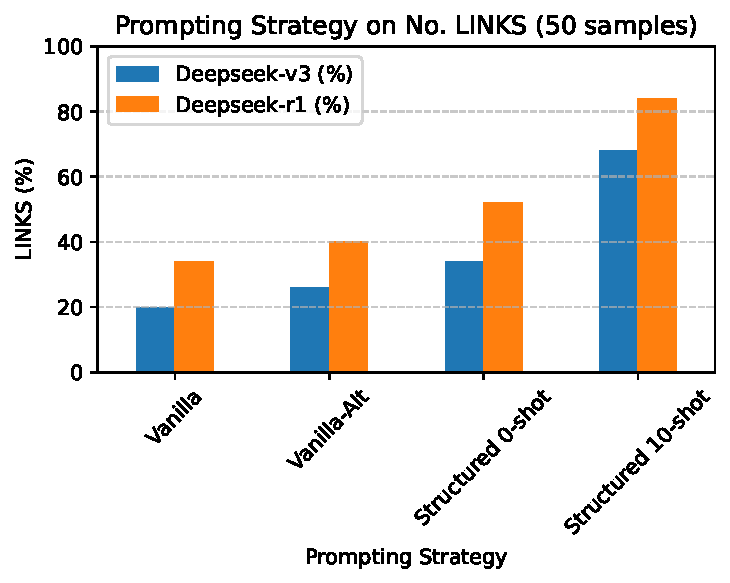
\includegraphics[width=\linewidth]{figures/prompt_comparison.pdf}
  \caption{Comparison of prompting methods (details in \Cref{app:prompt-usage}). Y-axis shows percentage of \lgms generated out of 50 requests sent for 50 vocabulary \vocab for each prompt $p$.}
  \label{fig:prompting-methods}
\end{figure}

As shown in \Cref{fig:prompting-methods}, \teachermodel consistently outperformed \xteachermodel across all prompting strategies, confirming our hypothesis that models specialized for reasoning tasks are better suited for linguistic analysis.

The vanilla prompt, which simply requested a \lgm for a vocabulary \vocab, produced \lgms in only 20\% of cases for \xteachermodel and 34\% for \teachermodel.

Changing the terminology from "mnemonic" to "memory cue" in increased the proportion of linguistically grounded responses to 26\% and 40\% respectively. We have a weak hypothesis that the word "mnemonic" may carry pre-training biases that associate it primarily with acronyms or simple keyword methods \citep{hackmannWordImportanceExplains2024}.

We also noted \teachermodel tended to generate lengthy, divergent reasoning traces, so we instructed it to stop analysis of linguistic features when it found a good enough mnemonic. When combining this instruction with structured output format, \xteachermodel produced \lgms in 35\% of cases, while \teachermodel achieved 52\%. This confirms that the model's performance didn't drop with shortened reasoning \citep{xuChainDraftThinking2025}, but further improved with explicit task instructions \citep{yinDidYouRead2023}.

The structured 10-shot CoT prompt, which included examples of linguistic reasoning before mnemonic generation, achieved the highest success rates of 68\% for \xteachermodel and 84\% for \teachermodel. This approach effectively guided the models to balance lingusitic grounding and memorability of mnemonics from the examples, preventing them from generating overly complex or abstract mnemonics.

Our qualitative analysis revealed several patterns in the generated mnemonics: \numlist{1} LLMs defaulted to surface-level associations rather than deeper linguistic analysis. \numlist{2} Both models favored etymology and morphology in their linguistic analysis, but they usually combined with phonetic or orthographic keywords in generated mnemonics \numlist{3} Several mnemonics are linguistically grounded but not memorable, despite the presence of both requirements in the prompt.

These findings indicated that while LLMs possess substantial linguistic knowledge for English language accessible through appropriate prompting, they benefit from structured guidance to apply this knowledge effectively for mnemonic generation. The strongest performance from CoT prompting suggested that reasoning elicitation is crucial for high-quality, linguistically grounded mnemonics.

Based on these insights, we selected the 10-shot CoT prompting approach to generate our synthetic dataset for model distillation, as described in the next section.
